\chapter{Analisi Attiva dei Log con il Modello IA ollama:qwen3.5}

In aggiunta al modello di sicurezza basato su Hyperledger Fabric e all'architettura in cui login, audit e logging sono gestiti direttamente sulla Blockchain, il sistema prevede un livello di analisi intelligente dei log che supporta il monitoraggio e la risposta alle anomalie.

Il modello \textbf{ollama:qwen3.5} viene utilizzato come componente di "analisi attiva" dei log, ossia un modulo IA che esamina in modo proattivo i dati generati dal sistema e produce indicazioni utili per l'operatore e per le eventuali contromisure.

\section{Integrazione nell'Infrastruttura}

L'integrazione di \texttt{ollama:qwen3.5} avviene su un livello di osservabilità e analisi dei log che interagisce con i seguenti componenti:

\begin{itemize}
    \item \textbf{Security Gateway (Flask):} Genera eventi di audit, richieste API, errori di autenticazione e accessi alle risorse protette.
    \item \textbf{Modulo di Logging:} Raccoglie le tracce dal backend e dalle API e le convoglia verso il sistema di analisi.
    \item \textbf{Modello IA ollama:qwen3.5:} Riceve i log strutturati e non strutturati, esegue l'analisi del contenuto, individua pattern sospetti e assegna livelli di gravità.
    \item \textbf{Dashboard di Sicurezza / Alerting:} Mostra i risultati dell'analisi e i consigli prodotti dall'IA, consentendo una risposta rapida e documentata.
\end{itemize}

Il modello non agisce come componente di controllo diretto sulla Blockchain, ma come strumento di supporto decisionale e di rilevazione delle anomalie nel perimetro applicativo e infrastrutturale.

\newpage
\subsection{Flusso Operativo}

L'analisi attiva dei log segue un flusso tipico in cui i dati vengono processati e interpretati da \texttt{ollama:qwen3.5}:

\begin{enumerate}
    \item \textbf{Raccolta:} I log sono generati dal backend Flask, dal modulo di autenticazione JWT, dai servizi REST e dalle operazioni di interazione diretta con la Blockchain, dove sono registrati gli eventi di login e di controllo.
    \item \textbf{Normalizzazione:} Il logging system converte i messaggi in un formato leggibile e strutturato, preservando timestamp, endpoint, identità utente e contesto operativo.
    \item \textbf{Analisi con IA:} Il modello Qwen 3.5 esamina le sequenze di log, ricerca anomalie, correlazioni e pattern comuni a attacchi noti.
    \item \textbf{Classificazione della Severità:} Ogni evento viene valutato e categorizzato con un livello di gravità, ad esempio \textit{Low}, \textit{Medium}, \textit{High} o \textit{Critical}.
    \item \textbf{Output e Consigli:} Il modello produce suggerimenti operativi, possibili cause e ipotesi di attacco, che vengono inoltrati al team o alla dashboard di monitoraggio.
\end{enumerate}

\section{Come l'IA Aiuta l'Analisi dei Log}

L'approccio basato su \texttt{ollama:qwen3.5} supporta l'analisi attiva dei log con i seguenti benefici:

\begin{itemize}
    \item \textbf{Rilevazione dei pattern sospetti:} Il modello è in grado di identificare schemi ripetuti e anomalie che possono sfuggire all'analisi manuale, ad esempio ripetuti tentativi di login falliti, richieste non autorizzate o payload malformati.
    \item \textbf{Livelli di severità definiti:} Assegna a ciascun evento un giudizio di gravità, rendendo più immediata la prioritarizzazione delle indagini.
    \item \textbf{Indicazioni sulle possibili cause:} Per ogni segnale anomalo, l'IA suggerisce una lista di cause probabili, come un attacco di brute force, un tentativo di SQL injection, un abuso dell'endpoint API o una configurazione errata.
    \item \textbf{Suggerimenti di intervento:} Vengono prodotti consigli concreti, ad esempio l'isolamento di una sessione sospetta, il blocco temporaneo di un IP o la revisione dei controlli di input.
    \item \textbf{Supporto per la risposta agli incidenti:} Il modello aiuta a trasformare il log grezzo in informazioni utili per il team, accelerando l'individuazione del problema e la sua mitigazione.
\end{itemize}

\newpage
\section{Addestramento sulla Baseline e Prompt del Modello}

Il modello \texttt{ollama:qwen3.5} è un modello preaddestrato. Nell'architettura del sistema, questo componente viene "allineato" alla baseline dei log del progetto tramite un prompt specifico che fornisce il contesto e le regole operative. In questo modo, ogni chiamata al modello include informazioni sul dominio del sistema, sulla struttura dei log e sui possibili scenari d'attacco.

La baseline viene definita come il comportamento atteso del sistema in condizioni normali: accessi corretti, transazioni blockchain valide, rifiuti di autenticazione legittimi e operazioni di query standard sulla rete Fabric. Il prompt viene aggiornato periodicamente in base ai nuovi pattern di log e alle minacce individuate in esercizi di security assessment.

Un esempio di prompt passato al modello ad ogni chiamata è il seguente:

\begin{lstlisting}[caption={Prompt inviato a ollama:qwen3.5 per l'analisi dei log},basicstyle=\scriptsize\ttfamily, breaklines=true]

        You are an AI security analyst monitoring the 'BuySellChain' platform.

        CRITICAL INSTRUCTIONS:
        1. Base your analysis STRICTLY AND ONLY on the provided logs.
        2. DO NOT hallucinate or assume events.
        3. Evaluate the logs against the System Baseline below.
        4. You MUST output EXACTLY ONE valid JSON object. If you detect multiple threats, AGGREGATE them into a single response, picking the highest severity and describing all of them in the 'explanation'.

        BUYSELLCHAIN SYSTEM BASELINE & KNOWN THREATS:
        - Normal Flows: Standard browser navigation, login, and bidding are normal. The canonical seller flow is Login -> Create Asset -> Create Auction The canonical buyer flow is Login -> Browse Auctions -> Place Bid.
        - Unauthorized Access: Accessing protected routes (e.g., /auctions/create, /assets, /admin) without authentication, or bypassing the frontend, is a severe anomaly.
        - Suspicious User Agents: Requests originating from tools like 'curl', 'sqlmap', 'Nmap', or non-standard browsers strongly indicate automated scripts, bots, or penetration testing.
        - Credential Stuffing / Brute Force: Anomalous spikes in POST requests to /auth/login. If the logs show multiple failed login attempts (at least 5) or a high volume of login requests from the same IP, this is a strong indicator of credential stuffing or brute force attacks.
        - Enumeration: Anomalous spikes in GET requests to /admin/users.
        - DoS / Overflood: Sudden spikes in POST requests to /bids, /auctions, or /assets.
        - Injection / XSS: HTML tags, JS scripts in descriptions, or escape characters in JSON payloads indicate XSS or Command Injection.

        Return ONLY ONE JSON object with this exact shape:
        {{
          "severity": "INFO|LOW|MEDIUM|HIGH|ALERT|CRITICAL",
          "attack_type": "...",
          "confidence": 0.0,
          "explanation": "...",
          "reasoning": "...",
          "remediation": "..."
        }}

        Logs:
        {json.dumps(preprocessed_logs)}
        

\end{lstlisting}

% \begin{lstlisting}[language=json,caption={Prompt inviato a ollama:qwen3.5 per l'analisi dei log}]
% {
%     "system": "Sei un analista di sicurezza specializzato in sistemi blockchain permissioned e in monitoraggio di log applicativi.",
%     "user": "Ricevi eventi di log strutturati relativi a un backend Flask che autentica utenti con JWT, esegue richieste verso un ledger Hyperledger Fabric e registra ogni evento di accesso sulla Blockchain.",
%     "instruction": "Analizza il log e determina se il comportamento risulta essere anomalo oppure no. Fornisci una classificazione (Low, Medium, High, Critical), una possibile causa, e suggerimenti operativi per mitigare il rischio. Se il pattern sembra riconducibile a un attacco noto, indica anche il tipo di attacco potenziale.",
%     "baseline": "Client login success, normal smart contract invocation, valid transaction submission, expected authorization failures for invalid roles, occasional retry due to latency, no SQL database activity.",
%     "log_event": {
%         "timestamp": "2026-06-03T12:34:56Z",
%         "level": "ERROR",
%         "component": "auth",
%         "message": "Authentication failed for user 'alice' - invalid signature",
%         "context": {
%             "ip": "192.0.2.10",
%             "endpoint": "/api/v1/login",
%             "transaction_id": "tx123"
%         }
%     }
% }
% \end{lstlisting}

Ogni richiesta a \texttt{ollama:qwen3.5} include una descrizione del dominio, della baseline e del contesto operativo. In questo modo il modello non solo classifica l'evento, ma lo confronta con il comportamento atteso del sistema e valuta la coerenza con le regole di sicurezza definito per l'infrastruttura.

\subsection{Addestramento e Adattamento}

Il termine "addestramento" è usato qui in senso lato. Nel flusso reale, il modello non viene ri-addestrato da zero, ma viene adattato tramite prompt engineering e aggiornamento della baseline. Le aggiunte includono:

\begin{itemize}
    \item pattern di accesso legittimi e sospetti specifici per il sistema;
    \item tipologie di errori legate a invocazioni del ledger Fabric;
    \item regole di correlazione tra eventi di login, chiamate API e transazioni blockchain.
\end{itemize}

Questo approccio consente al sistema di sfruttare un modello preaddestrato mantenendo un comportamento contestualizzato per l'ambiente specifico di 
\texttt{BuySellChain}.

\subsection{Esempi di Tipologie di Eventi Analizzati}

\begin{itemize}
    \item \textbf{Autenticazione fallita ripetuta:} La sequenza di login falliti viene classificata come \textit{High} o \textit{Critical} a seconda della frequenza e della presenza di tentativi d'accesso a risorse sensibili.
    \item \textbf{Richieste API anomale:} Payload malformati o parametri sospetti vengono segnalati come possibili tentativi di injection o abuso di endpoint.
    \item \textbf{Errore di autorizzazione:} Accessi negati verso risorse protette possono indicare tentativi di escalation di privilegio o account compromessi.
    \item \textbf{Timeout e rallentamenti:} Prestazioni degradate associate a picchi improvvisi di traffico sono interpretati come possibili attacchi DDoS o stress operativo.
\end{itemize}

\section{Interfacciamento con l'Infrastruttura}

In termini di infrastruttura, il componente di log analysis può essere rappresentato come uno strato di osservabilità orizzontale che rileva eventi nelle seguenti aree:

\begin{itemize}
    \item \textbf{Frontend Web:} Errori di validazione lato client e anomalie nella comunicazione con il backend.
    \item \textbf{Backend Flask:} Eventi di autenticazione, autorizzazione, errori interni, eccezioni e metriche di performance.
    \item \textbf{Blockchain e Ledger:} Eventi di invocazione delle API del ledger, errori di invio delle transazioni, operazioni non valide rispetto allo Smart Contract e registrazione degli accessi.
\end{itemize}

In questo modo, il modello IA diventa un punto di 
\textit{situational awareness}, in grado di correlare informazioni provenienti da tutto il sistema e produrre un quadro d'insieme più ricco rispetto all'analisi isolata dei singoli log.

\begin{figure}[H]
    \centering
    \begin{tikzpicture}[node distance=1.8cm, >=Stealth, every node/.style={draw, rounded corners, align=center, text width=3.5cm, minimum height=1.1cm}]
        \node (frontend) {Frontend Web \\ (Browser)};
        \node[right=of frontend] (gateway) {Security Gateway \\ (Flask / JWT / API REST)};
        \node[right=of gateway] (blockchain) {Hyperledger Fabric \\ (Ledger, Auth, Audit)};
        \node[above=of gateway] (ia) {ollama:qwen3.5 \\ Log Analysis};
        \node[below=of gateway] (dashboard) {Dashboard di Sicurezza \\ Alert \& Severity};
        \draw[->, thick] (frontend) -- (gateway);
        \draw[->, thick] (gateway) -- (blockchain);
        \draw[<->, thick] (gateway) -- (ia);
        \draw[->, thick] (ia) -- (dashboard);
    \end{tikzpicture}
    \caption{Integrazione dell'analisi dei log basata su ollama:qwen3.5, in stile analogo a una figura di architettura a blocchi}
    \label{fig:ia_integration}
\end{figure}

\begin{figure}[H]
    \centering
    %\fbox{\parbox{0.9\textwidth}{\centering Spazio riservato per il diagramma dei livelli di severità e dei consigli generati}} 
    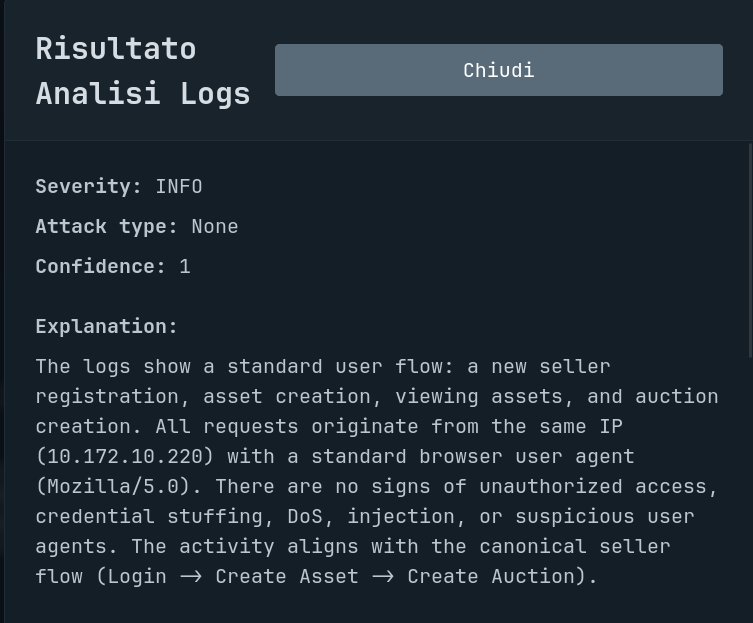
\includegraphics[width=0.7\textwidth]{images/analisi_log1.png}
    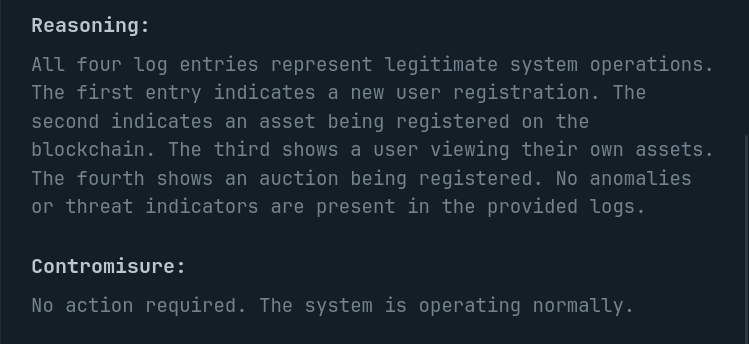
\includegraphics[width=0.7\textwidth]{images/analisi_log2.png}
    \caption{Esempio di output grafico dell'analisi attiva dei log - Flusso Standard}
    \label{fig:ia_output}
\end{figure}

\begin{figure}[H]
    \centering
    %\fbox{\parbox{0.9\textwidth}{\centering Spazio riservato per il diagramma dei livelli di severità e dei consigli generati}} 
    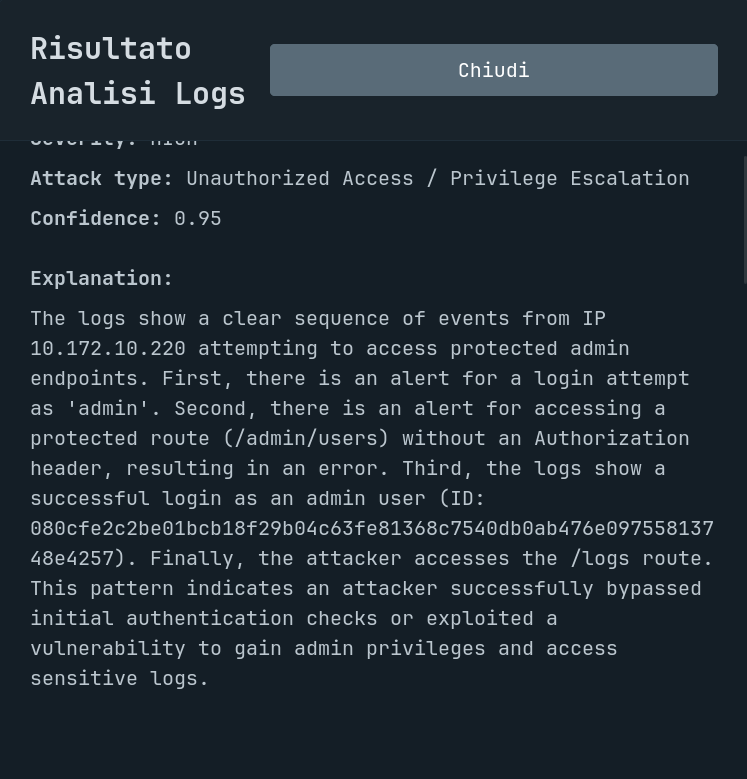
\includegraphics[width=0.7\textwidth]{images/analisi_log_Att1.png}
    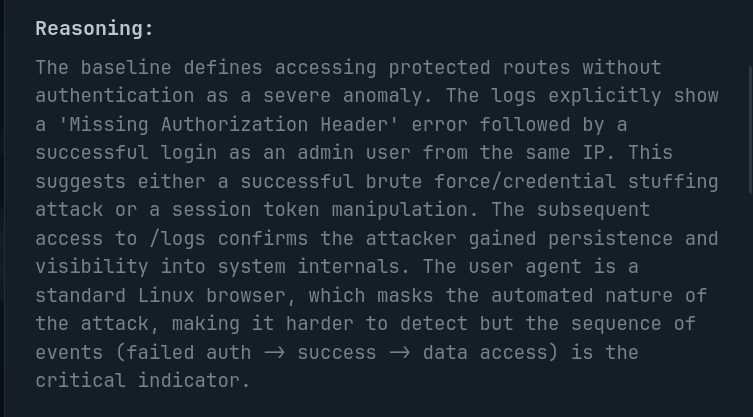
\includegraphics[width=0.7\textwidth]{images/analisi_log_att2.png}
    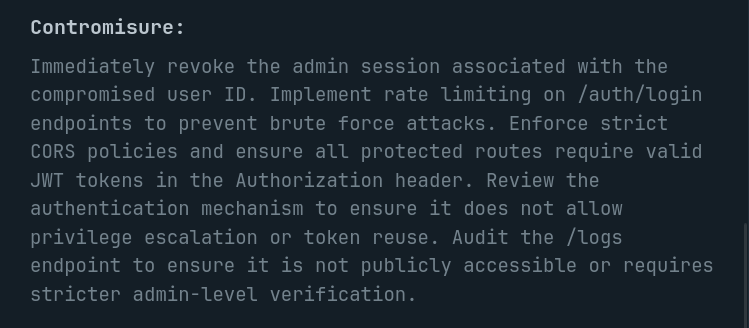
\includegraphics[width=0.7\textwidth]{images/analisi_log_att3.png}
    \caption{Esempio di output grafico dell'analisi attiva dei log - Flusso Anomalo/Attacco}
    \label{fig:ia_output}
\end{figure}

\section{Considerazioni sulla Sicurezza e Sul Ruolo dell'IA}

L'utilizzo di \texttt{ollama:qwen3.5} in questo contesto deve essere interpretato come un supporto all'analisi e non come un controllo di autorizzazione. Il modello fornisce:

\begin{itemize}
    \item \textbf{Insight qualitativi:} Aiuta a comprendere meglio il significato delle anomalie e a identificare possibili minacce emergenti.
    \item \textbf{Miglioramento continuo:} Può essere aggiornato con nuove regole e nuovi pattern di attacco, rendendo l'analisi più precisa nel tempo.
    \item \textbf{Riduzione del carico manuale:} Automatizza parte dell'interpretazione dei log, lasciando agli analisti umani il compito di decidere le azioni correttive più idonee.
\end{itemize}

L'approccio IA rende la gestione della sicurezza più proattiva, permettendo di anticipare gli incidenti prima che diventino compromissioni gravi dell'intero sistema.
